\section{Simulation and Performance}

The author compares the OBKF with the classic Kalman filter with known parameter, IBRKF, minimax Kalman filter, and MAP Kalman filter. To evaluate the estimation, the covariance of the estimation error is used. In the equation (\ref{eq:metric}), ${\bf P^x}_{k+1}(\bm{\theta};\bm{\theta}')$ is the covariance of the estimation error $\bm{x}_k-\bm{\hat x}_k$. 

\begin{align}\label{eq:metric}
{\bf P^x}_{k+1}(\bm{\theta};\bm{\theta}') &= \bm{\Phi}_k({\bf I}-{\bf K}^{\bm{\theta}'}_k{\bf H}_k){\bf P^x}_k(\bm{\theta};\bm{\theta}')({\bf I}-{\bf K}^{\bm{\theta}'}_k{\bf H}_k)^T\bm{\Phi}^T_k \nonumber \\
&\quad + \bm{\Gamma}_k{\bf Q}^{\theta_1}\bm{\Gamma}_k^T + \bm{\Phi}_k\bm{K}_k^{\bm{\theta}'}\bm{R}^{\theta_2}(\bm{K}_k^{\bm{\theta}'})^T\bm{\Phi}_k^T
\end{align}

The trace of ${\bf P^x}_{k+1}(\bm{\theta};\bm{\theta}')$ is computed as the MSE of the estimation, and it is used as the metric.

\subsection{Simulation of the algorithm}

To evaluate the performance of the OBKF, consider a tracking problem with an unknown parameter. To the equations (\ref{eq:linear1}) and (\ref{eq:linear2}), substitute the following parameters.

\begin{align*}
    &\bm{\Phi}_k=
    \begin{bmatrix}
        1 & \tau & 0 & 0\\
        0 & 1 & 0 & 0 \\
        0 & 0 & 1 & \tau \\
        0 & 0 & 0 & 1 \\
    \end{bmatrix}, \;\;
    \bm{H}_k = 
    \begin{bmatrix}
        1&0&0&1\\
        0&0&1&0
    \end{bmatrix}, \;\;
    \bm{\Gamma}_k = \bm{I} \\
    &\bm{Q} = q \times 
    \begin{bmatrix}
        \tau^3/3 & \tau^2/2 & 0 & 0 \\
        \tau^2/2 & \tau & 0 & 0 \\
        0 & \tau & 0 & 0 \\
        0 & 0 & \tau^2/2 & \tau
    \end{bmatrix}, \;\;
    \bm{R}=r\times\begin{bmatrix}
        1&0\\
        0&1
    \end{bmatrix}
\end{align*}

Here, $\tau$ is the measurement interval. $q$ and $r$ are the covariance noise intensity.

In the simulation, the author uses $\tau = 1$ second. The initial conditions are set as $\E[\bm{x}_0]=[100\, 10\, 30\, -10]^T$ and ${\rm cov}[\bm{x}_0]={\rm diag}([25\, 2\, 25\, 2])$ where ${\rm diag}(v)$ is a diagonal matrix whose diagonal elements are $v$.
The parameter $q$ is set to 2 and $r$ is defined as a random variable. As for the unknown parameter $q$ and $r$, $q$ is assumed as known, and $r$ is uniformly distributed over [0.25,4]. 

\begin{figure}[H]
    \begin{center}
    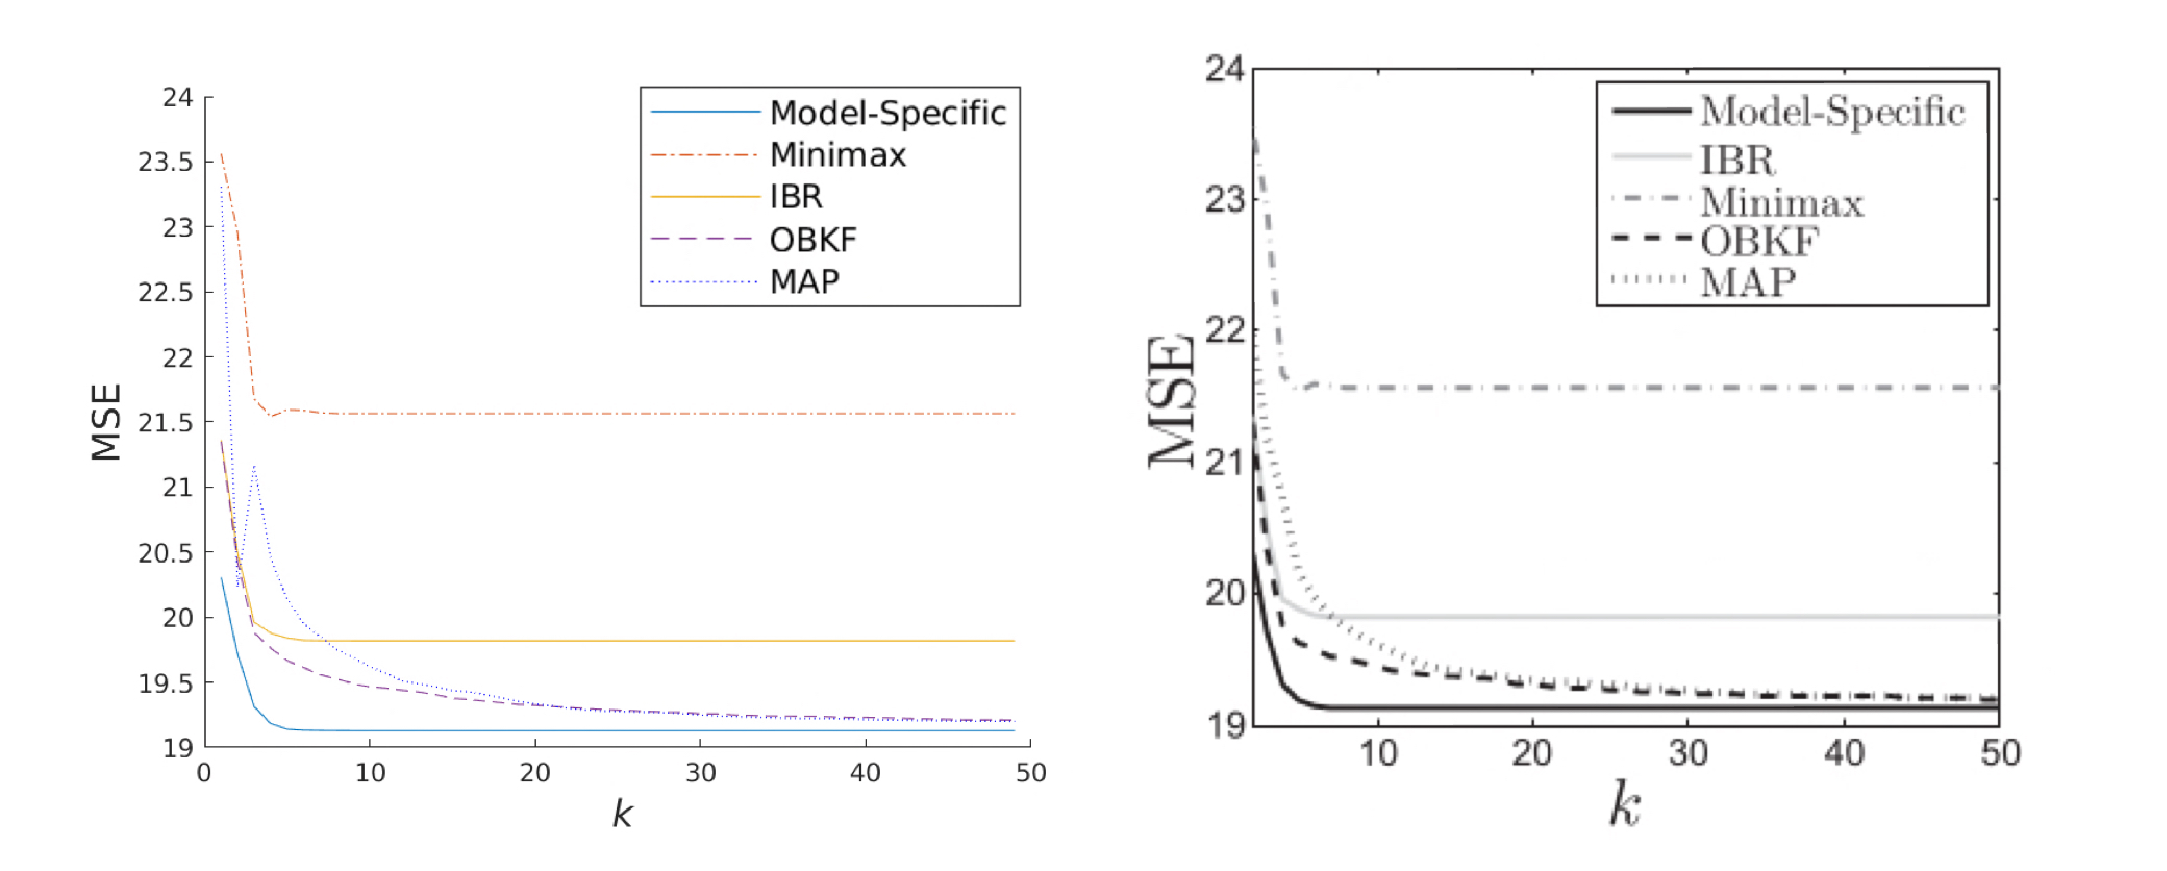
\includegraphics[width=9.5cm]{img/r1_mse.eps}
    \caption{caption}
    \label{fig:label}
    \end{center}
\end{figure}

\begin{figure}[H]
    \begin{center}
    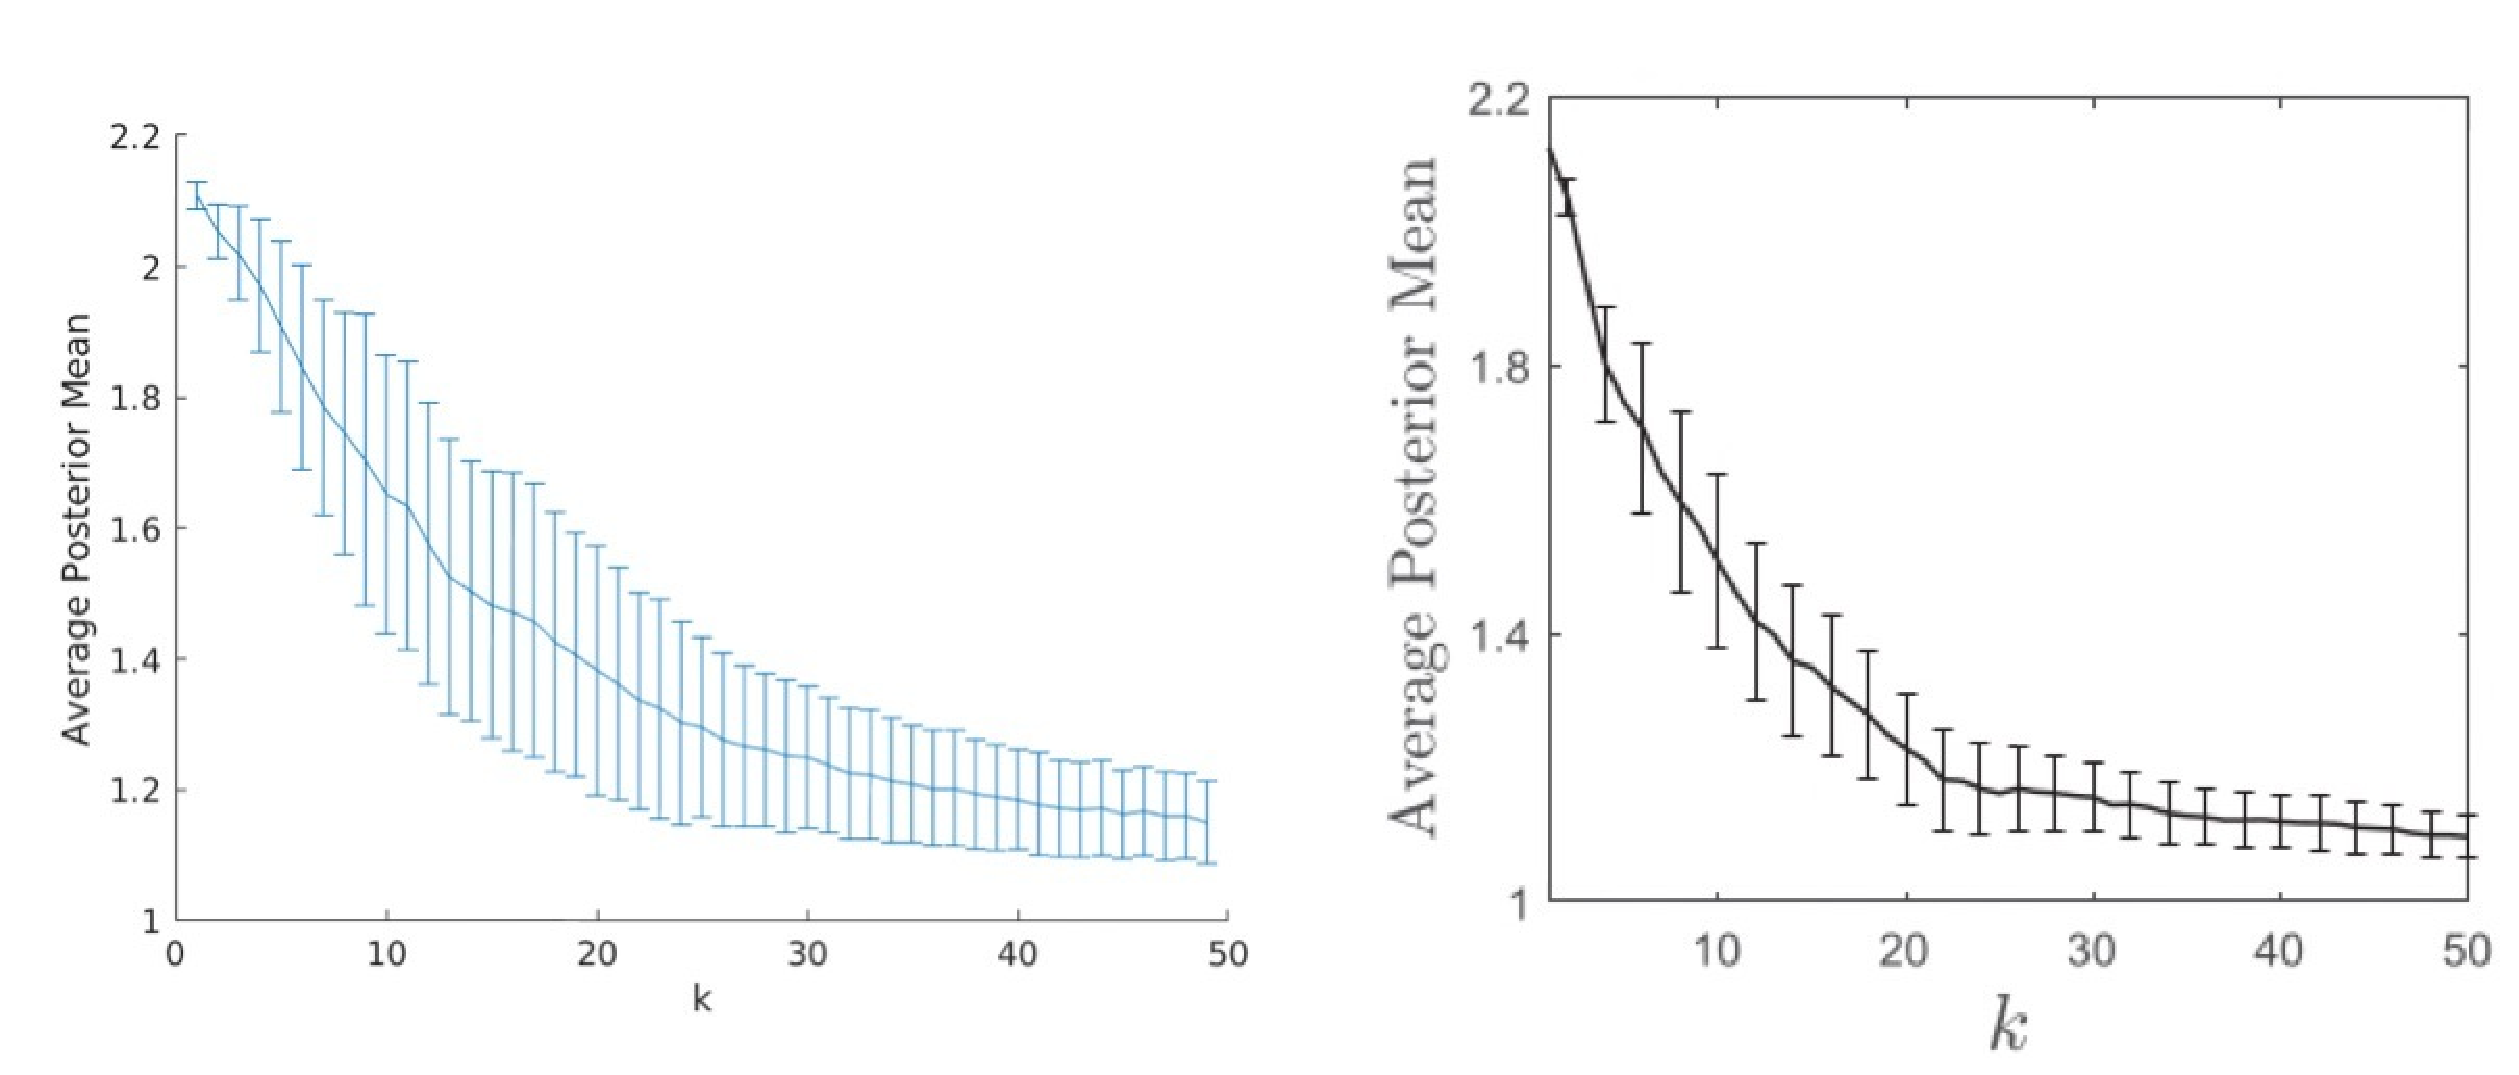
\includegraphics[width=9.5cm]{img/r1_mean.eps}
    \caption{caption}
    \label{fig:label}
    \end{center}
\end{figure}

Fig. compares the simulated MSE with the figure from the paper. You can see that in the both images, the OBKF outperforms the other Kalman filters.

Fig. compares the estimated $r$ in the simulation and the figure from the paper. In the both image, the estimated $r$ converges to the true value $r=1$ as k increases.
